\newpage

\section*{ $^{197}$Au(n,$\gamma$)$^{198}$Au }

Power Level: 100 kW(th) \\
Time at Power: 60.0 s \\
Wait Time:  2.0 h \\
Counting Time:  2.0 m \\
Total Activity at Removal: 5.01e+01 $\mu Ci$

\begin{table*}[h]
\centering
\begin{tabular}{ |c|c|c|c|c|c| }
 \hline
 Position & Mass $mg$ & Counting Activity $\mu Ci$ & Area (Counts) & Error \% \\
 \hline 
 1 & 4.10 & 1.07e+01 & 2.14e+06 & 0.0683 \\ 
\hline
 2 & 4.10 & 1.54e+01 & 3.08e+06 & 0.0570 \\ 
\hline
 3 & 4.30 & 1.51e+01 & 3.02e+06 & 0.0576 \\ 
\hline
 4 & 4.20 & 8.06e+00 & 1.61e+06 & 0.0787 \\ 
\hline
\end{tabular}
\end{table*}

\begin{figure}[h]
\centering
\begin{subfigure}{.5\textwidth}
  \centering
     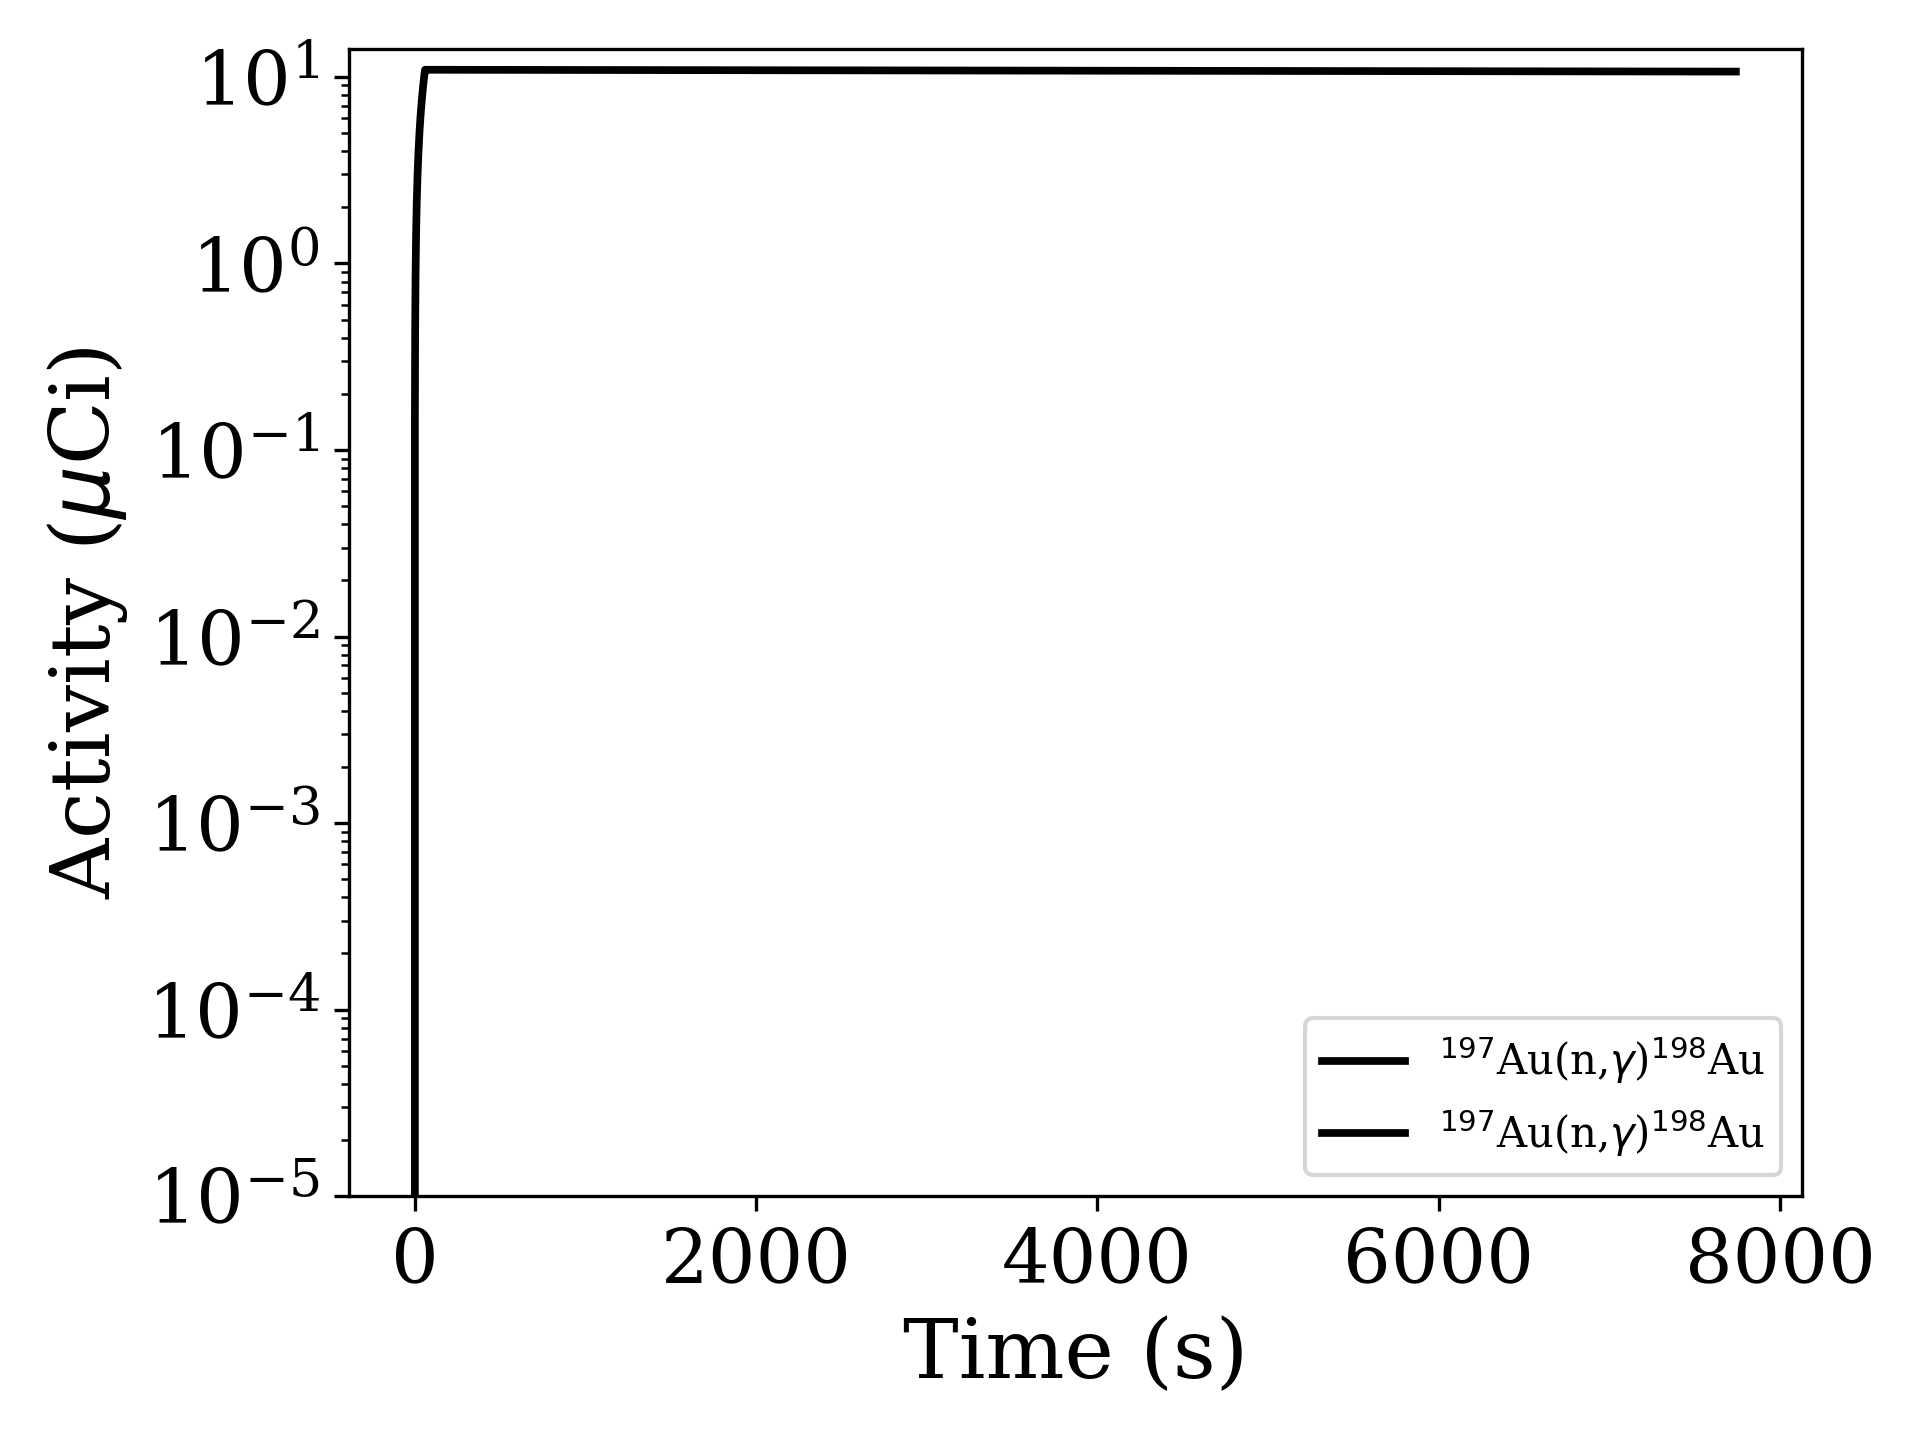
\includegraphics[width=.8\textwidth]{plot/Au-197(n,gamma)Au-198_wisconsin1} 

  \caption{Activity}
\end{subfigure}%
\begin{subfigure}{.5\textwidth}
  \centering
     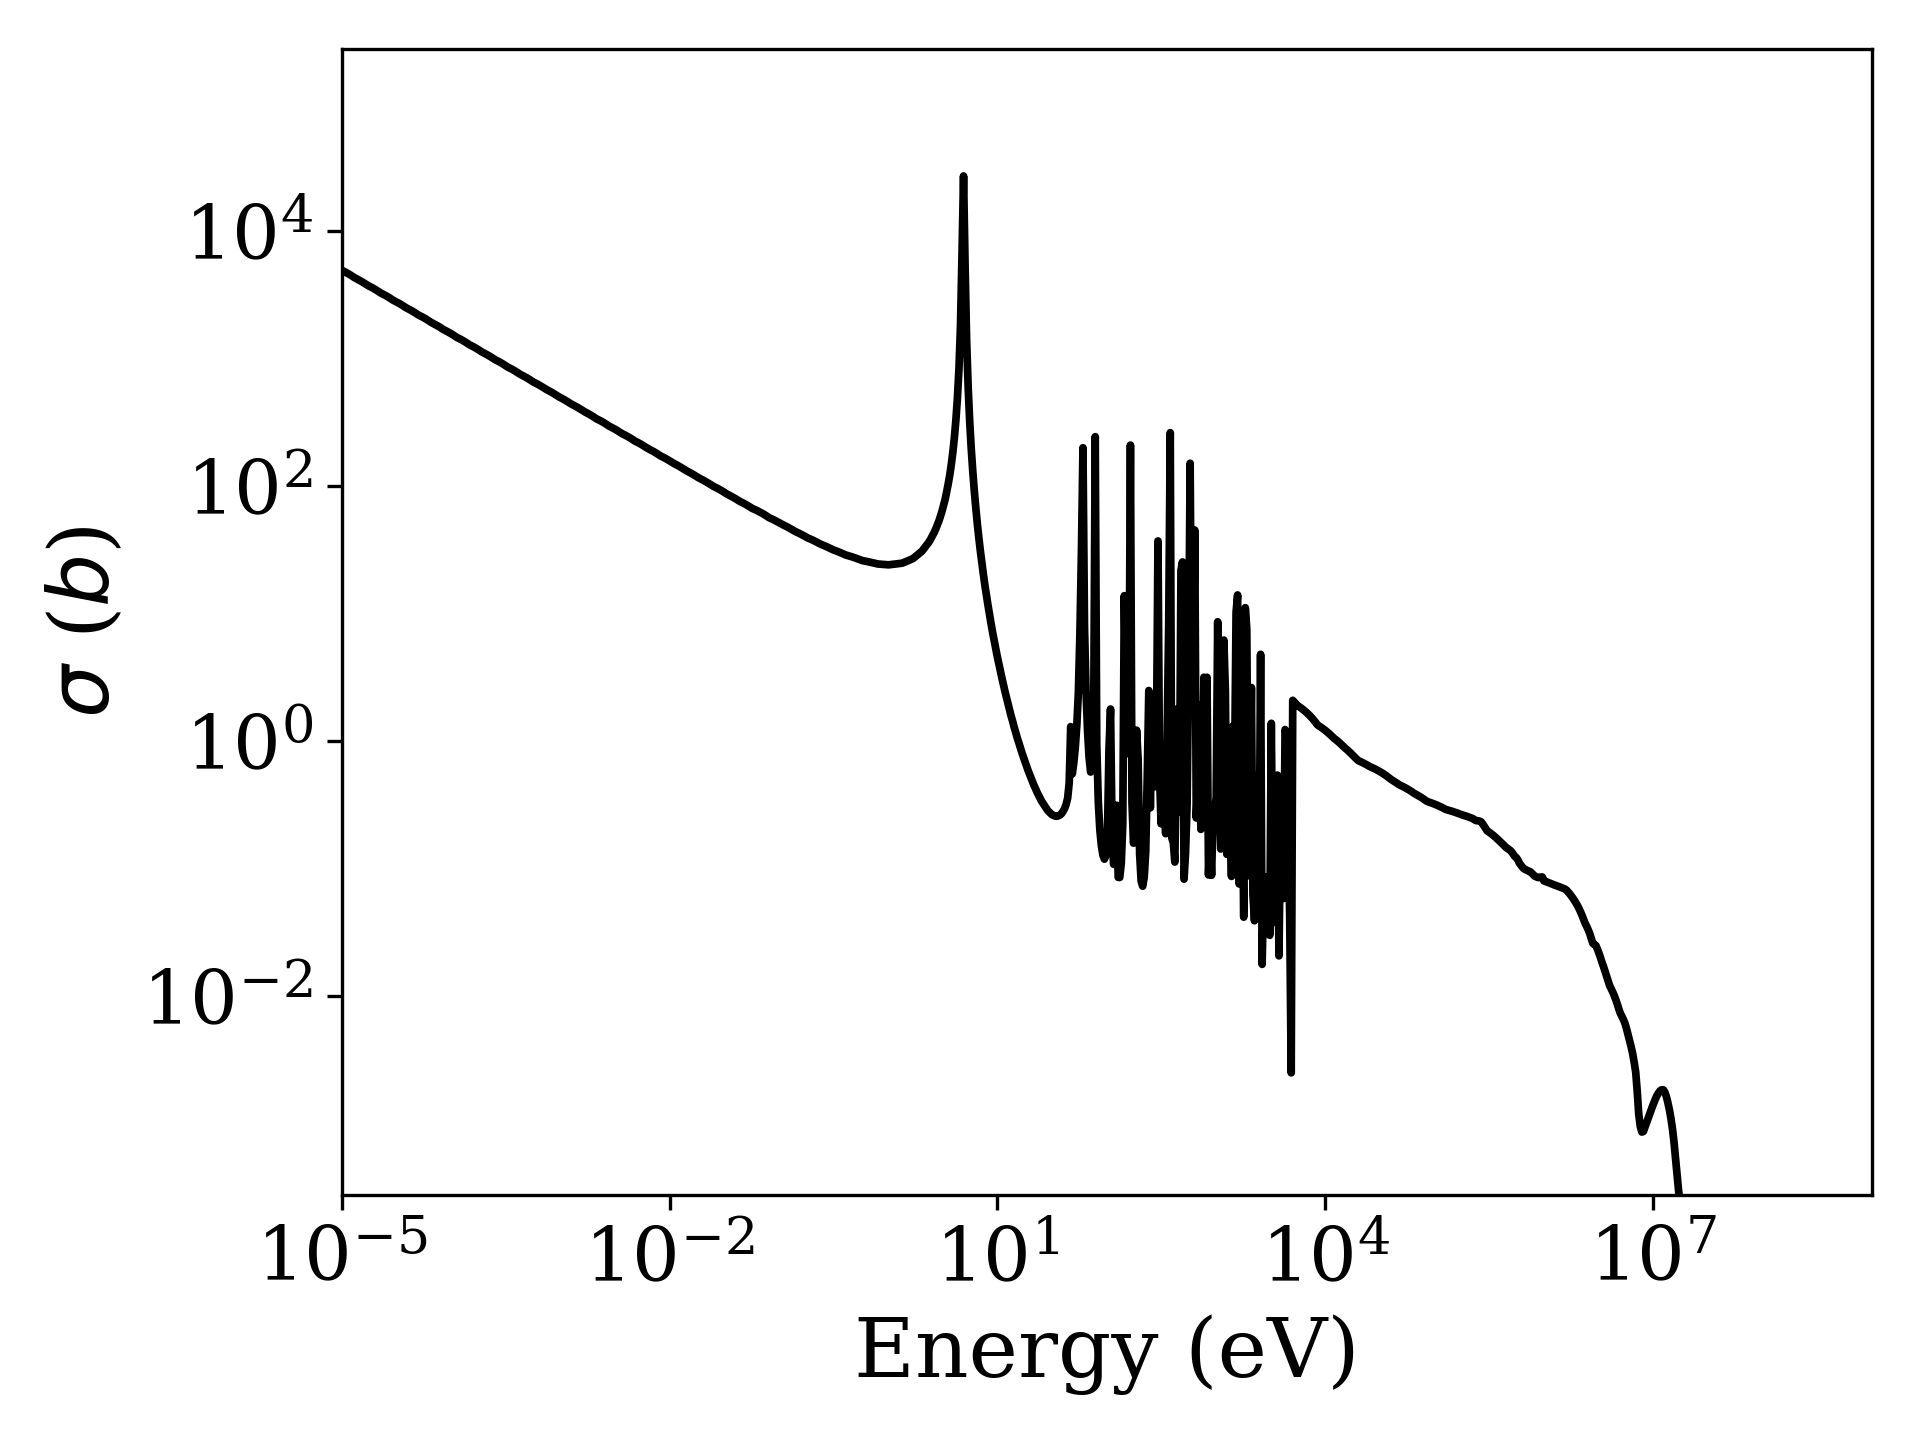
\includegraphics[width=.8\textwidth]{plot/Au-197(n,gamma)Au-198} 

  \caption{Cross Section}
\end{subfigure}
\end{figure}

\begin{table*}[h]
\centering
\begin{tabular}{ |c|c|c|c|c|c|c| }
 \hline
 Reaction & T$_{1/2}$ & ROI (eV) & Important Gammas (keV) \\
 \hline 
 $^{197}$Au(n,$\gamma$)$^{198}$Au &  2.7 d & 1.31e-02, 5.46e+00 & 412(0.95) \\ 
\hline
\end{tabular}
\end{table*}
